\documentclass[aspectratio=169,hyperref=unicode]{beamer}

\usepackage[absolute,overlay]{textpos}
\usepackage{graphicx}
\usepackage{adjustbox}
\usepackage{chemfig}
\usepackage{makecell}
\usepackage[version=4]{mhchem}
\usepackage{wrapfig}
\usepackage{multirow}
\adjustboxset*{center}
\usepackage{caption}
\usepackage{chemformula}
\usepackage{elements}

%dělení slov
\usepackage{ragged2e}
\let\raggedright=\RaggedRight
%konec dělení slov

\usepackage{fontspec}
\usepackage{unicode-math}

\usepackage{polyglossia}
\setdefaultlanguage{czech}

\def\uv#1{„#1“}

\usetheme[numbering=fraction]{metropolis}
%\mode<presentation>{\usetheme{Madrid}}
%\DefineNamedColor{named}{pozadi}{RGB}{200,200,200}
%\usecolortheme{crane}

%------------------------------------------------
% Fonty (LuaLaTeX nebo XeLaTeX) %------------------------------------------------
\usepackage{fontspec}
\setmainfont{Source Sans Pro}
\setsansfont{Source Sans Pro}
\setmonofont{JetBrains Mono}

%------------------------------------------------
% Grafika
%------------------------------------------------
\usepackage{graphicx}
\usepackage{booktabs}
\usepackage{multirow}
\usepackage{tikz}
\usetikzlibrary{ positioning, arrows.meta, calc, shapes.geometric }

%------------------------------------------------
% Barvy
%------------------------------------------------
\definecolor{MUblue}{HTML}{00467F}
\definecolor{MUlight}{HTML}{EAF2F8}
\definecolor{MUgreen}{HTML}{008A5E}
\setbeamercolor{frametitle}{fg=MUblue}
\setbeamercolor{title}{fg=MUblue}
\setbeamercolor{block title}{ fg=white, bg=MUlight }
\setbeamercolor{block body}{ bg=MUblue }
\setbeamercolor{alerted text}{ fg=MUgreen }

%------------------------------------------------
% Metropolis nastavení
%------------------------------------------------

\metroset{ progressbar=frametitle, sectionpage=progressbar, block=fill }

%------------------------------------------------
% Vzhled seznamů
%------------------------------------------------
\setbeamertemplate{itemize item}{\small$\blacktriangleright$} \setbeamertemplate{itemize subitem}{\tiny$\blacktriangleright$}

%------------------------------------------------
% Číslování obrázků a tabulek %------------------------------------------------

\setbeamertemplate{caption}[numbered]

% --------------------------------------------------
% Bez navigačních ikon
% --------------------------------------------------

\setbeamertemplate{navigation symbols}{}

% --------------------------------------------------
% Horní lišta se sekcí
% --------------------------------------------------

\setbeamercolor{section in head/foot}{ fg=white, bg=MUgreen } \setbeamertemplate{headline}
{ \leavevmode
	\hbox{ \begin{beamercolorbox}[ wd=\paperwidth, ht=2.8ex, dp=1.2ex, leftskip=1em ]{section in head/foot}
			\insertsectionhead

			\ifx\insertsubsectionhead\empty \else \insertsectionhead\hspace{1em}$\triangleright$\hspace{0.5em} \insertsubsectionhead \fi

		\end{beamercolorbox}
	}
}

% --------------------------------------------------
% Dolní lišta s číslováním
% --------------------------------------------------

\setbeamercolor{author in head/foot}{ fg=white, bg=MUgreen } \setbeamertemplate{footline}
{
	\leavevmode
	\hbox{
		\begin{beamercolorbox}[ wd=\paperwidth, ht=2.8ex, dp=1.2ex, rightskip=1em ]{author in head/foot}
			\hfill
			\insertframenumber/\inserttotalframenumber \end{beamercolorbox}
	}
}
\begin{document}

\title[Crisis] % (optional, only for long titles)
{Vyhodnocování IR a RA spekter}

\author % (optional, for multiple authors)
{Zdeněk Moravec, Ústav chemie, PřF MU \\ hugo@chemi.muni.cz \\
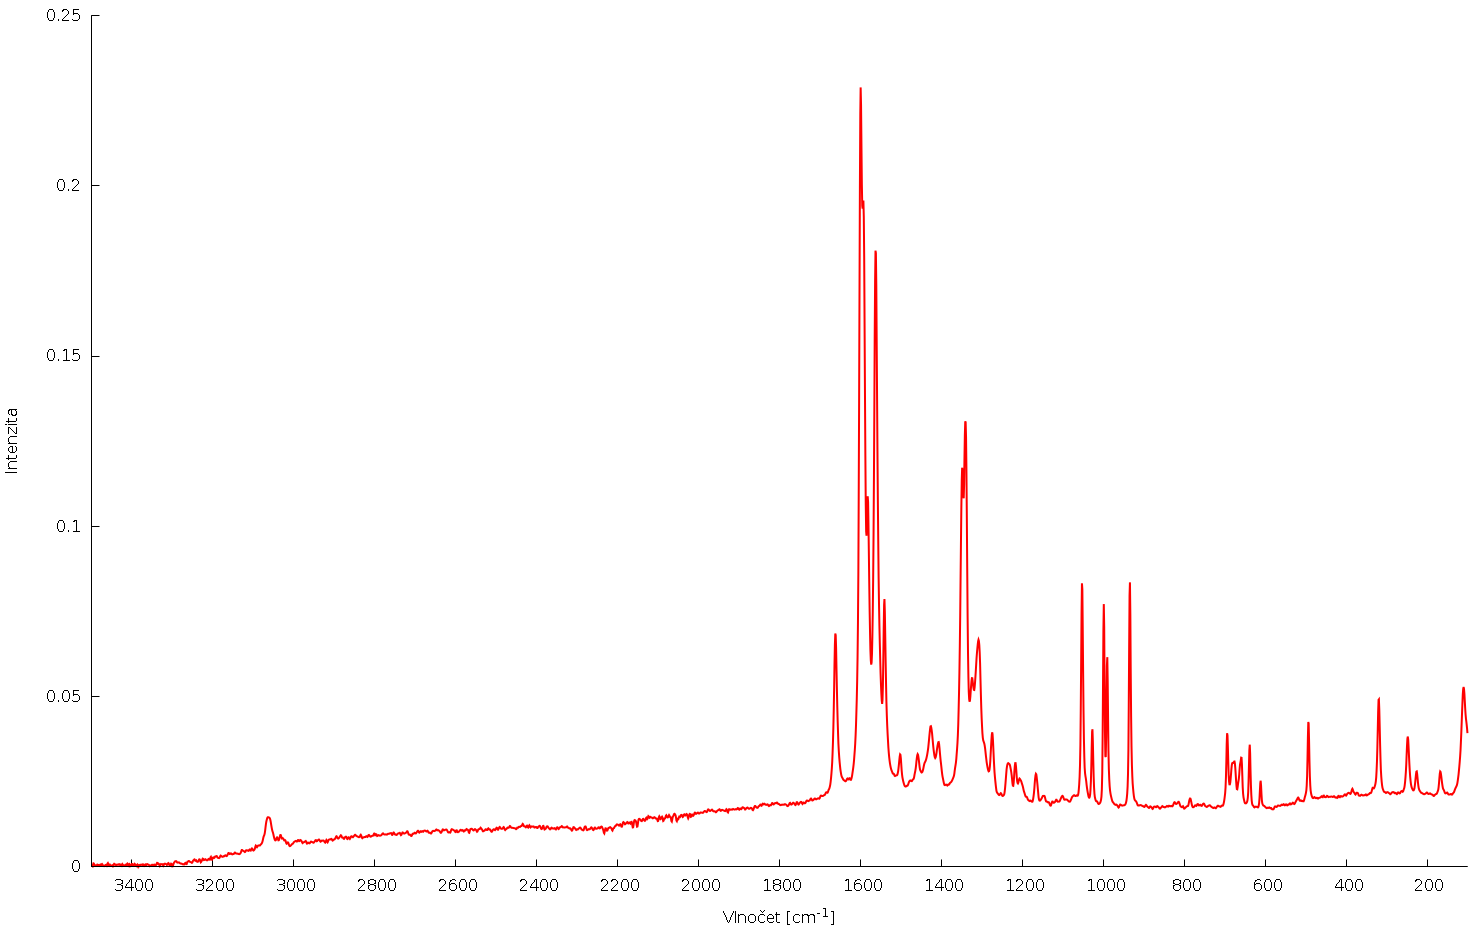
\includegraphics[width=60mm]{img/raman-spect.png}}
%{http://z-moravec.net}

\date{ } %hide date on titlepage

%\subtitle{Metody chemické výzkumu}

\frame{\titlepage}

\section{Úvod}
\frame{
	\frametitle{}
	\vfill
	\begin{itemize}
		\item Vzorky, u kterých neznáme ani přibližné složení, lze pomocí IR a RA spektroskopie analyzovat s využitím databází spekter.
		\item Pokud máme alespoň přibližnou představu o struktuře vzorku, lze spektra využít pro potvrzení nebo vyvrácení přítomnosti funkčních skupin a pro kontrolu čistoty reaktantů a produktů.
	\end{itemize}
	\begin{center}
	\adjincludegraphics[width=115mm]{img/irBandsOrg.png}
	\end{center}
	\vfill
}

\section{Kvalitativní analýza}
\subsection{Rozdělení oblastí spekter}
\frame{
	\frametitle{}
	\vfill
	\begin{itemize}
	\item  NIR (0,7 -- 2,5 $\mu$m; 14 000 - 4 000 cm$^{-1}$) - infračervená spektroskopie v blízké oblasti -- převážně overtony a kombinační vibrace. Intenzita pásů je nižší než v MIR oblasti a pásy se často překrývají.
	\item  \textbf{MIR} (2,5 -- 25 $\mu$m; 4 000 - 400 cm$^{-1}$) - infračervená spektroskopie ve střední oblasti -- základní vibrace molekul.
	\item  FIR (25 -- 1000 $\mu$m; 400 - 10 cm$^{-1}$) - infračervená spektroskopie ve vzdálené oblasti -- vibrace vazeb kov-halogen, deformační vibrace skeletu molekul.
	\end{itemize}
	\vfill
}

\subsection{Databáze spekter}
\frame{
	\frametitle{}
	\vfill
	\begin{itemize}
		\item Pokud známe předpokládané složení vzorku, je možné využít databáze spekter a provést srovnání spektra našeho vzorku s tabelovaným spektrem.
		\item Je vhodné, aby byla obě spektra naměřená stejnou technikou.
		\item Databáze jsou často placené nástroje, které umožňují vyhledávání a srovnávání spekter.
		\item Databáze dostupné bez poplatku umožňují zpravidla pouze prohlížení spekter.
	\end{itemize}
	\vfill
}

\frame{
	\frametitle{}
	\vfill
	\begin{itemize}
		\item \href{http://sdbs.riodb.aist.go.jp/sdbs/cgi-bin/cre\_index.cgi}{sdbs.riodb.aist.go.jp/sdbs/cgi-bin/cre\_index.cgi}
	\end{itemize}
	\adjincludegraphics[height=.8\textheight]{img/sdbs.png}
	\vfill
}

\frame{
	\frametitle{}
	\vfill
	\begin{itemize}
		\item \href{http://sdbs.riodb.aist.go.jp/sdbs/cgi-bin/cre\_index.cgi}{sdbs.riodb.aist.go.jp/sdbs/cgi-bin/cre\_index.cgi}
	\end{itemize}
	\adjincludegraphics[height=.8\textheight]{img/sdbs2.png}
	\vfill
}

\frame{
	\frametitle{}
	\vfill
	\begin{itemize}
		\item \url{http://webbook.nist.gov/chemistry/}
	\end{itemize}
	\adjincludegraphics[height=.8\textheight]{img/nist.png}
	\vfill
}

\frame{
	\frametitle{}
	\vfill
	\begin{itemize}
		\item \url{http://webbook.nist.gov/chemistry/}
	\end{itemize}
	\adjincludegraphics[height=.8\textheight]{img/nist2.png}
	\vfill
}

\subsection{Základní pravidla pro interpretaci vibračních spekter}
\frame{
	\frametitle{}
	\vfill
	\begin{enumerate}
		\item Pokud známe alespoň přibližnou strukturu vzorku, je možné provést interpretaci s využitím charakteristických frekvencí funkčních skupin.
		\item Poloha absorpčního pásu charakteristické skupiny bývá často ovlivněna okolím molekuly jen omezeně, a proto se nachází v relativně úzké oblasti vlnočtů.
	\end{enumerate}
	\begin{center}
	\adjincludegraphics[width=100mm]{img/irBandsOrg.png}
	\end{center}
	\vfill
}

\frame{
	\frametitle{}
	\vfill
	\begin{enumerate}
		\item  Nejprve se podívejte na oblast vyšších vlnočtů ($>$1500 cm$^{-1}$) a hledejte výrazné pásy.
		\item  Pro každý významný pás si připravte seznam možných přiřazení.
		\item  Oblast nižších vlnočtů použijte pro potvrzení nebo vyvrácení přítomnosti funkčních skupin.
		\item \textit{Nesnažte se přiřadit každý pás ve spektru.}
		\item Pokud je to možné, hledejte pro každou funkční skupinu více pásů, např. aldehydy by měly mít pás okolo 1730~cm$^{-1}$ a zároveň i pás v oblasti 2900-2700~cm$^{-1}$. Pokud některý z pásů chybí, skupina pravděpodobně ve struktuře přítomna není.
		\item Intenzity pásů berte v úvahu pouze orientačně.
		\item \textit{V závislosti na technice měření a stavu vzorku (kapalný, pevný, roztok) může docházet k malým změnám v poloze pásů.}
		\item Pozor na pásy náležející rozpouštědlu.
	\end{enumerate}
	\vfill
}

\subsection{Interpretace vibračních spekter organických sloučenin}
\frame{
	\frametitle{}
	\vfill
	\begin{itemize}
	\item 4000-2500 cm$^{-1}$ oblast valenčních vibrací X-H
	\item 2500-2000 cm$^{-1}$ oblast trojných vazeb
	\item 2000-1500 cm$^{-1}$ oblast dvojných vazeb
	\item 1500-600 cm$^{-1}$ oblast otisku prstu (fingerprint)
	\end{itemize}
	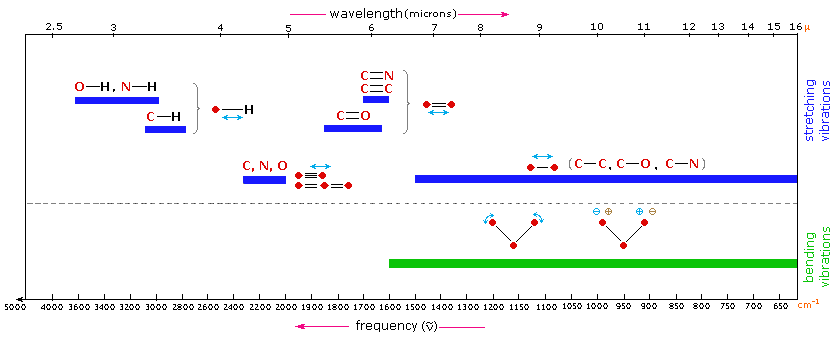
\includegraphics[width=85mm]{img/irBandsOrg.png}
	\vfill
}

\frame{
	\frametitle{}
	\vfill
	\adjincludegraphics[width=115mm,valign=l]{img/tab.png}
	\vfill
}

\frame{
	\frametitle{}
	\vfill
	\begin{tabular}{|l|l|l|l|l|l|}
	\hline
	\textbf{Sloučenina} & \textbf{Skupina} & \textbf{Vlnočet [cm$^{-1}$]}
	& \textbf{Sloučenina} & \textbf{Skupina} & \textbf{Vlnočet [cm$^{-1}$]} \\\hline
	\multirow{3}{*}{Alkany} & \ce{C-H} & 2850-3000 & \multirow{3}{*}{Karboxylové kys.} & \ce{C=O} & 1700-1725 \\
	& \ce{C-C} & 800-1000 & & \ce{O-H} & 2500-3300 \\
	& & & & \ce{C-O} & 1100-1300 \\\hline
	\multirow{2}{*}{Aromáty} & \ce{C-H} & 3000-3100 & \multirow{2}{*}{Aldehydy} & \ce{C=O} & 1720-1740 \\
	& \ce{C=C} & 1450-1600 & & \ce{C-H} & 2700-2900 \\\hline
	\multirow{2}{*}{Alkeny} & \ce{C-H} & 3080-3140 &
	\multirow{2}{*}{Alkoholy} & \ce{O-H} & 3300-3600 \\
	& \ce{C=C} & 1630-1670 & & \ce{C-O} & 1050-1200 \\\hline
	\end{tabular}
	\vfill
}

\frame{
	\frametitle{}
	\vfill
	\begin{enumerate}
		\item Absorpční pásy v oblasti 3200--2700~cm$^{-1}$ prokazují přítomnost alifatických (pod 3000~cm$^{-1}$) nebo aromatických (nad 3000~cm$^{-1}$) \ce{C-H} vazeb.
		\item Absorpční pásy v oblasti 3650--3250~cm$^{-1}$ prokazují přítomnost \ce{O-H} a \ce{N-H} vazeb.
		\item Absorpční pásy v oblasti 1850--1650~cm$^{-1}$ prokazují přítomnost \ce{C=O} vazeb. V této oblasti může docházet k interferenci s vazbami \ce{C=N} a \ce{N=N}, např. v purinech a azo- sloučeninách.
		\item Absorpční pásy v oblasti 1670--1620~cm$^{-1}$ prokazují přítomnost alifatických, nenasycených \ce{C=C} vazeb. Zároveň by měl být přítomen absorpční pás o vlnočtu vyšším než 3000~cm$^{-1}$.
		\item Absorpční pásy v oblasti 1615--1495~cm$^{-1}$, společně s absorpčním pásem o vlnočtu vyšším než 3000~cm$^{-1}$ prokazují přítomnost aromatických vazeb.
		\item Absorpční pásy v oblasti 2300--1990~cm$^{-1}$, často indikují přítomnost trojných nebo kumulovaných násobných vazeb.
	\end{enumerate}
	\vfill
}

\subsubsection{Aromatické sloučeniny}
\frame{
	\frametitle{}
	\vfill
	\begin{tabular}{|l|l|}
	\hline
	\textbf{Vibrace} & \textbf{Vlnočet [cm$^{-1}$]} \\\hline
	\ce{C-H} arom. valenční & 3100-3000 \\\hline
	\ce{C-H} alif. valenční & 3000-2900 \\\hline
	Kombinační, overtony & 2000-1700 \\\hline
	\ce{C=C} & 1650-1430 \\\hline
	\ce{C-H} deformační v rovině kruhu & 1275-1000 \\\hline
	\ce{C-H} deformační mimo rovinu kruhu & 900-690 \\\hline
	\end{tabular}
	\begin{columns}
	\column{.8\textwidth}
	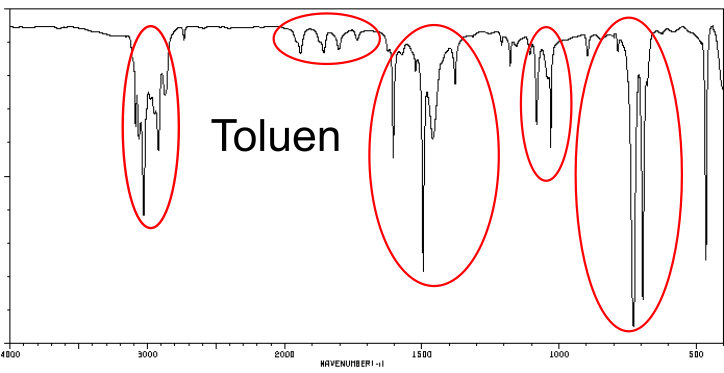
\includegraphics[width=75mm]{img/toluene.png}
	\column{.18\textwidth}
	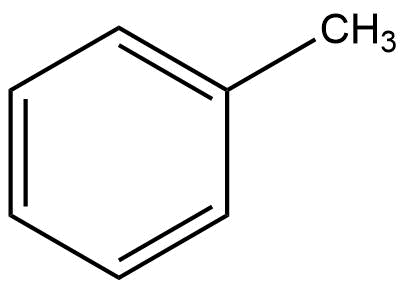
\includegraphics[width=26mm]{img/toluene-struct.png}
	\end{columns}
	\vfill
}

\subsection{Anorganické sloučeniny}
\frame{
	\frametitle{}
	\vfill
	\begin{itemize}
		\item Spektra anorganických sloučenin zpravidla obsahují méně pásů, ty jsou širší a nalézáme je i na nižších vlnočtech, často až ve FIR oblasti.
		\item Látky obsahující pouze iontovou vazbu, např. NaCl, nevykazují v MIR oblasti fundamentální molekulové vibrace; pozorovatelné jsou pouze nízkofrekvenční mřížkové vibrace.
		\item Stupeň hydratace sloučeniny ovlivňuje vzhled spektra.
	\end{itemize}
	\begin{figure}
		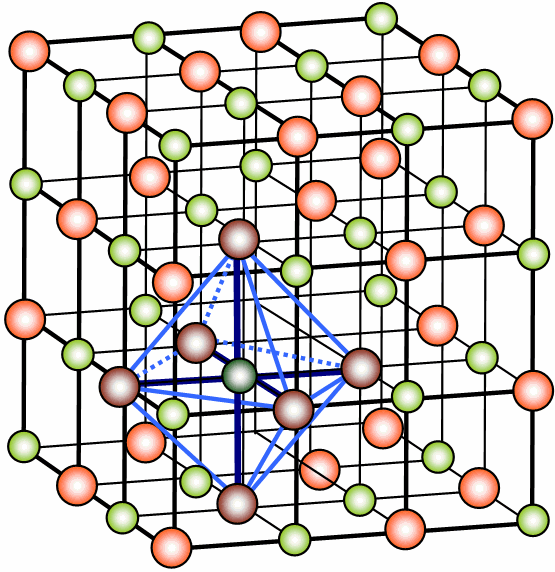
\includegraphics[height=.45\textheight]{img/NaCl.png}
	\end{figure}
	\vfill
}

\frame{
	\frametitle{}
	U anorganických sloučenin mají polohy pásů výrazně větší závislost na struktuře a koordinaci než u běžných organických funkčních skupin.

	\begin{columns}
	\begin{column}{0.4\textwidth}
	\begin{tabular}{|l|l|}
	\hline
	\textbf{Ion} & \textbf{Vlnočet [cm$^{-1}$]} \\\hline
	\multirow{2}{*}{\ce{CO$_3^{2-}$}} & 1450-1410 \\
	& 880-800 \\\hline
	\multirow{2}{*}{\ce{SO$_4^{2-}$}} & 1130-1080 \\
	& 680-610 \\\hline
	\multirow{2}{*}{\ce{NO$_3^{-}$}} & 1410-1340 \\
	& 860-800 \\\hline
	\ce{PO$_4^{3-}$} & 1100-950 \\\hline
	\ce{SiO$_4^{4-}$} & 1100-900 \\\hline
	\multirow{2}{*}{\ce{NH$_4^{+}$}} & 3335-3030 \\
	& 1485-1390 \\\hline
	\end{tabular}
	\end{column}

	\begin{column}{0.6\textwidth}
	\begin{tabular}{|l|l|}
		\hline
		\textbf{Vibrace} & \textbf{Vlnočet [cm$^{-1}$]} \\\hline
		$\nu$(S=O) & \multirow{2}{*}{1500--1000} \\
		$\nu(S-O)$ & \\\hline
		$\nu(S-F)$ & 900--600 \\\hline
		$\delta(O-S-O)$ & 700--400 \\\hline
		$\nu(S-Cl)$ & 600--400 \\\hline
		$\nu(S-Br)$ & 400--300 \\\hline
		$\nu(P=O)$ & 1500--1200 \\\hline
		$\nu(P-O)$ & 1200--900 \\\hline
		$\nu(P-F)$ & 1000--700 \\\hline
		$\nu(P-Cl)$ & 600--400 \\\hline
		$\delta(O-P-O)$ & 650--300 \\\hline
	\end{tabular}
	\vfill
	\end{column}
	\end{columns}
}

\frame{
	\frametitle{}
	\vfill
	\begin{center}
		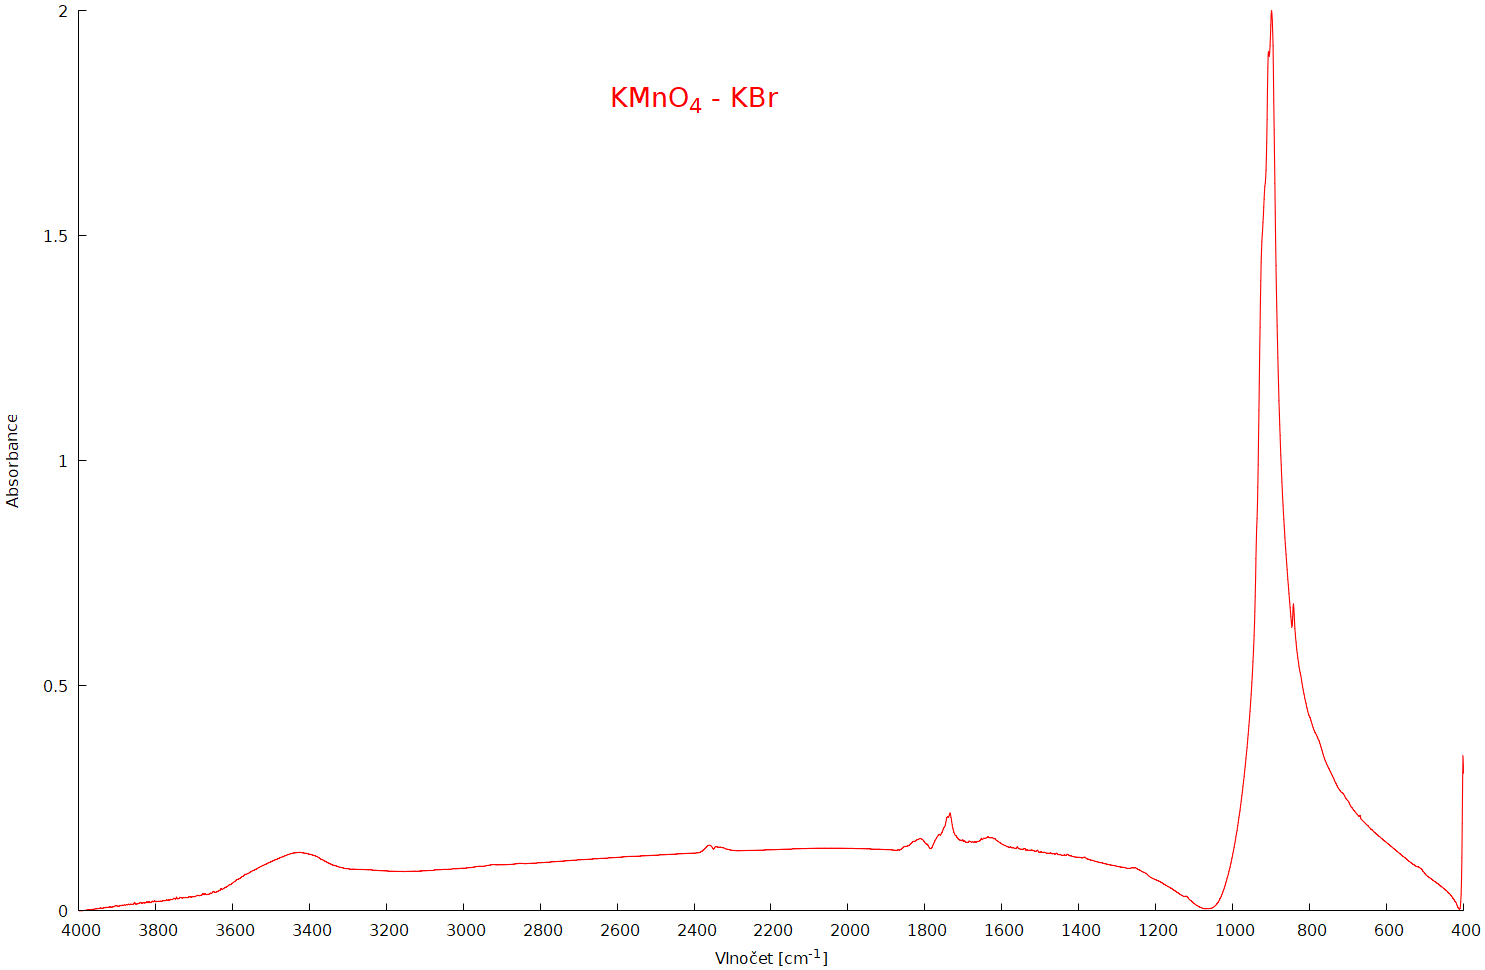
\includegraphics[height=.85\textheight]{spectra/200410/KMnO4-KBr.png}
	\end{center}
	\vfill
}

\subsection{Faktory ovlivňující polohu absorpčního pásu}
\frame{
	\frametitle{}
	\vfill
	\begin{itemize}
		\item Vodíkové vazby.
		\item Izotopická substituce.
		\item Hmotnost atomů tvořících vazbu.
	\end{itemize}
	\begin{center}
	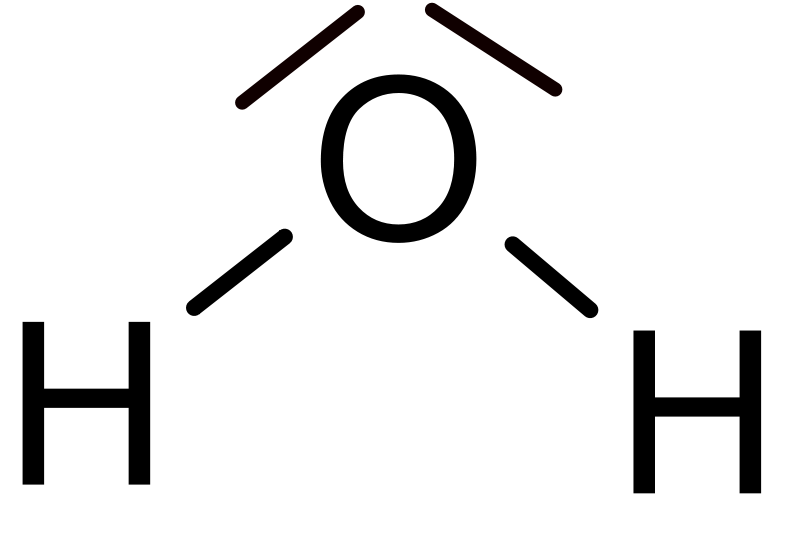
\includegraphics[height=0.2\textheight]{img/H2O.png}
	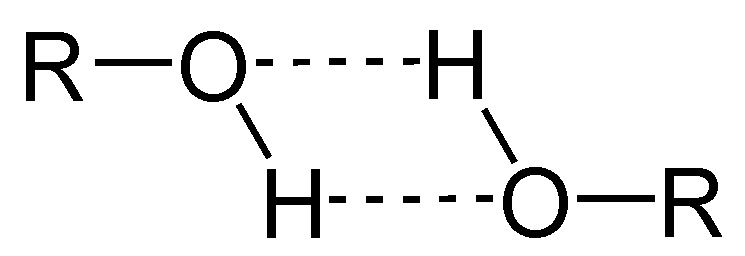
\includegraphics[height=0.2\textheight]{img/H-bonding_alcohol.png}
	\end{center}
	\vfill
}

\subsection{Vodíkové vazby}
\frame{
	\frametitle{}
	\vfill
	\begin{itemize}
		\item Přítomnost intra-\ i intermolekulárních vodíkových vazeb ovlivňuje sílu vazby a tím i polohu odpovídajícího pásu ve spektru.
		\item Se vzrůstající teplotou dochází k oslabování vodíkových vazeb a tím k posunu odpovídajících pásů k vyšším hodnotám vlnočtu.
	\end{itemize}
	\begin{columns}
		\column{.8\textwidth}
		\begin{table}[H]
			\caption*{Závislost vlnočtu vibrace OH skupiny fenolu na koncentraci dioxanu v \ce{CCl4}\footnotemark[1]}
			\begin{tabular}{|r@{,}l|l|l|l|}
				\hline
				\multicolumn{2}{|l|}{Konc. dioxanu [\%]} & $\nu_{OH}$ & $\nu_{OH}$ fenol-dioxan & $\Delta\nu$ \\\hline
				0 & 0 & 3611 & - & - \\\hline
				2 & 3 & 3612 & 3377 & 234 \\\hline
				22 & 1 & 3610 & 3365 & 246 \\\hline
				72 & 5 & - & 3347 & 264 \\\hline
				100 & 0 & - & 3338 & 273 \\\hline
			\end{tabular}
		\end{table}
		\column{.25\textwidth}
		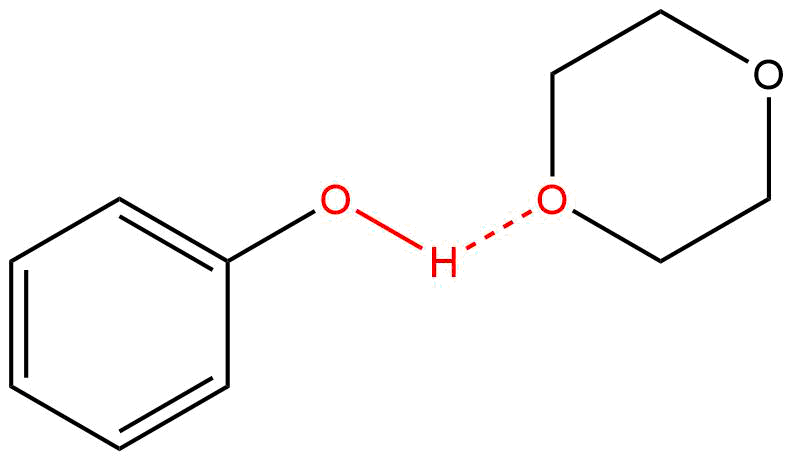
\includegraphics[width=28mm]{img/phenol-dioxane.png}
	\end{columns}
	\footnotetext[1]{\href{http://dx.doi.org/10.1021/ja00887a001}{\emph{J. Am. Chem. Soc.}, \textbf{1963}, \emph{85} (4), 371--380}}
	\vfill

}

\subsection{Izotopická substituce}
\frame{
	\frametitle{}
	\vfill
	\begin{columns}
		\begin{column}{0.5\textwidth}
			\begin{itemize}
				\item Izotopická substituce usnadňuje interpretaci vibračních spekter
				\item Nedochází ke změně geometrie molekuly, ale změní se hmotnost atomů a tím i poloha absorpčních pásů
				\item 	$\nu = \frac{1}{2\pi}\sqrt{\frac{k}{\mu}}; \mu = \frac{m_1m_2}{(m_1 + m_2)}$
				\begin{itemize}
					\item k - silová konstanta vazby
					\item $\mu$ - redukovaná hmotnost
					\item $m_1, m_2$ - hmotnosti atomů
				\end{itemize}
				\item Těžší izotop způsobuje posun pásu k nižším vlnočtům
			\end{itemize}
		\end{column}

		\begin{column}{0.5\textwidth}
			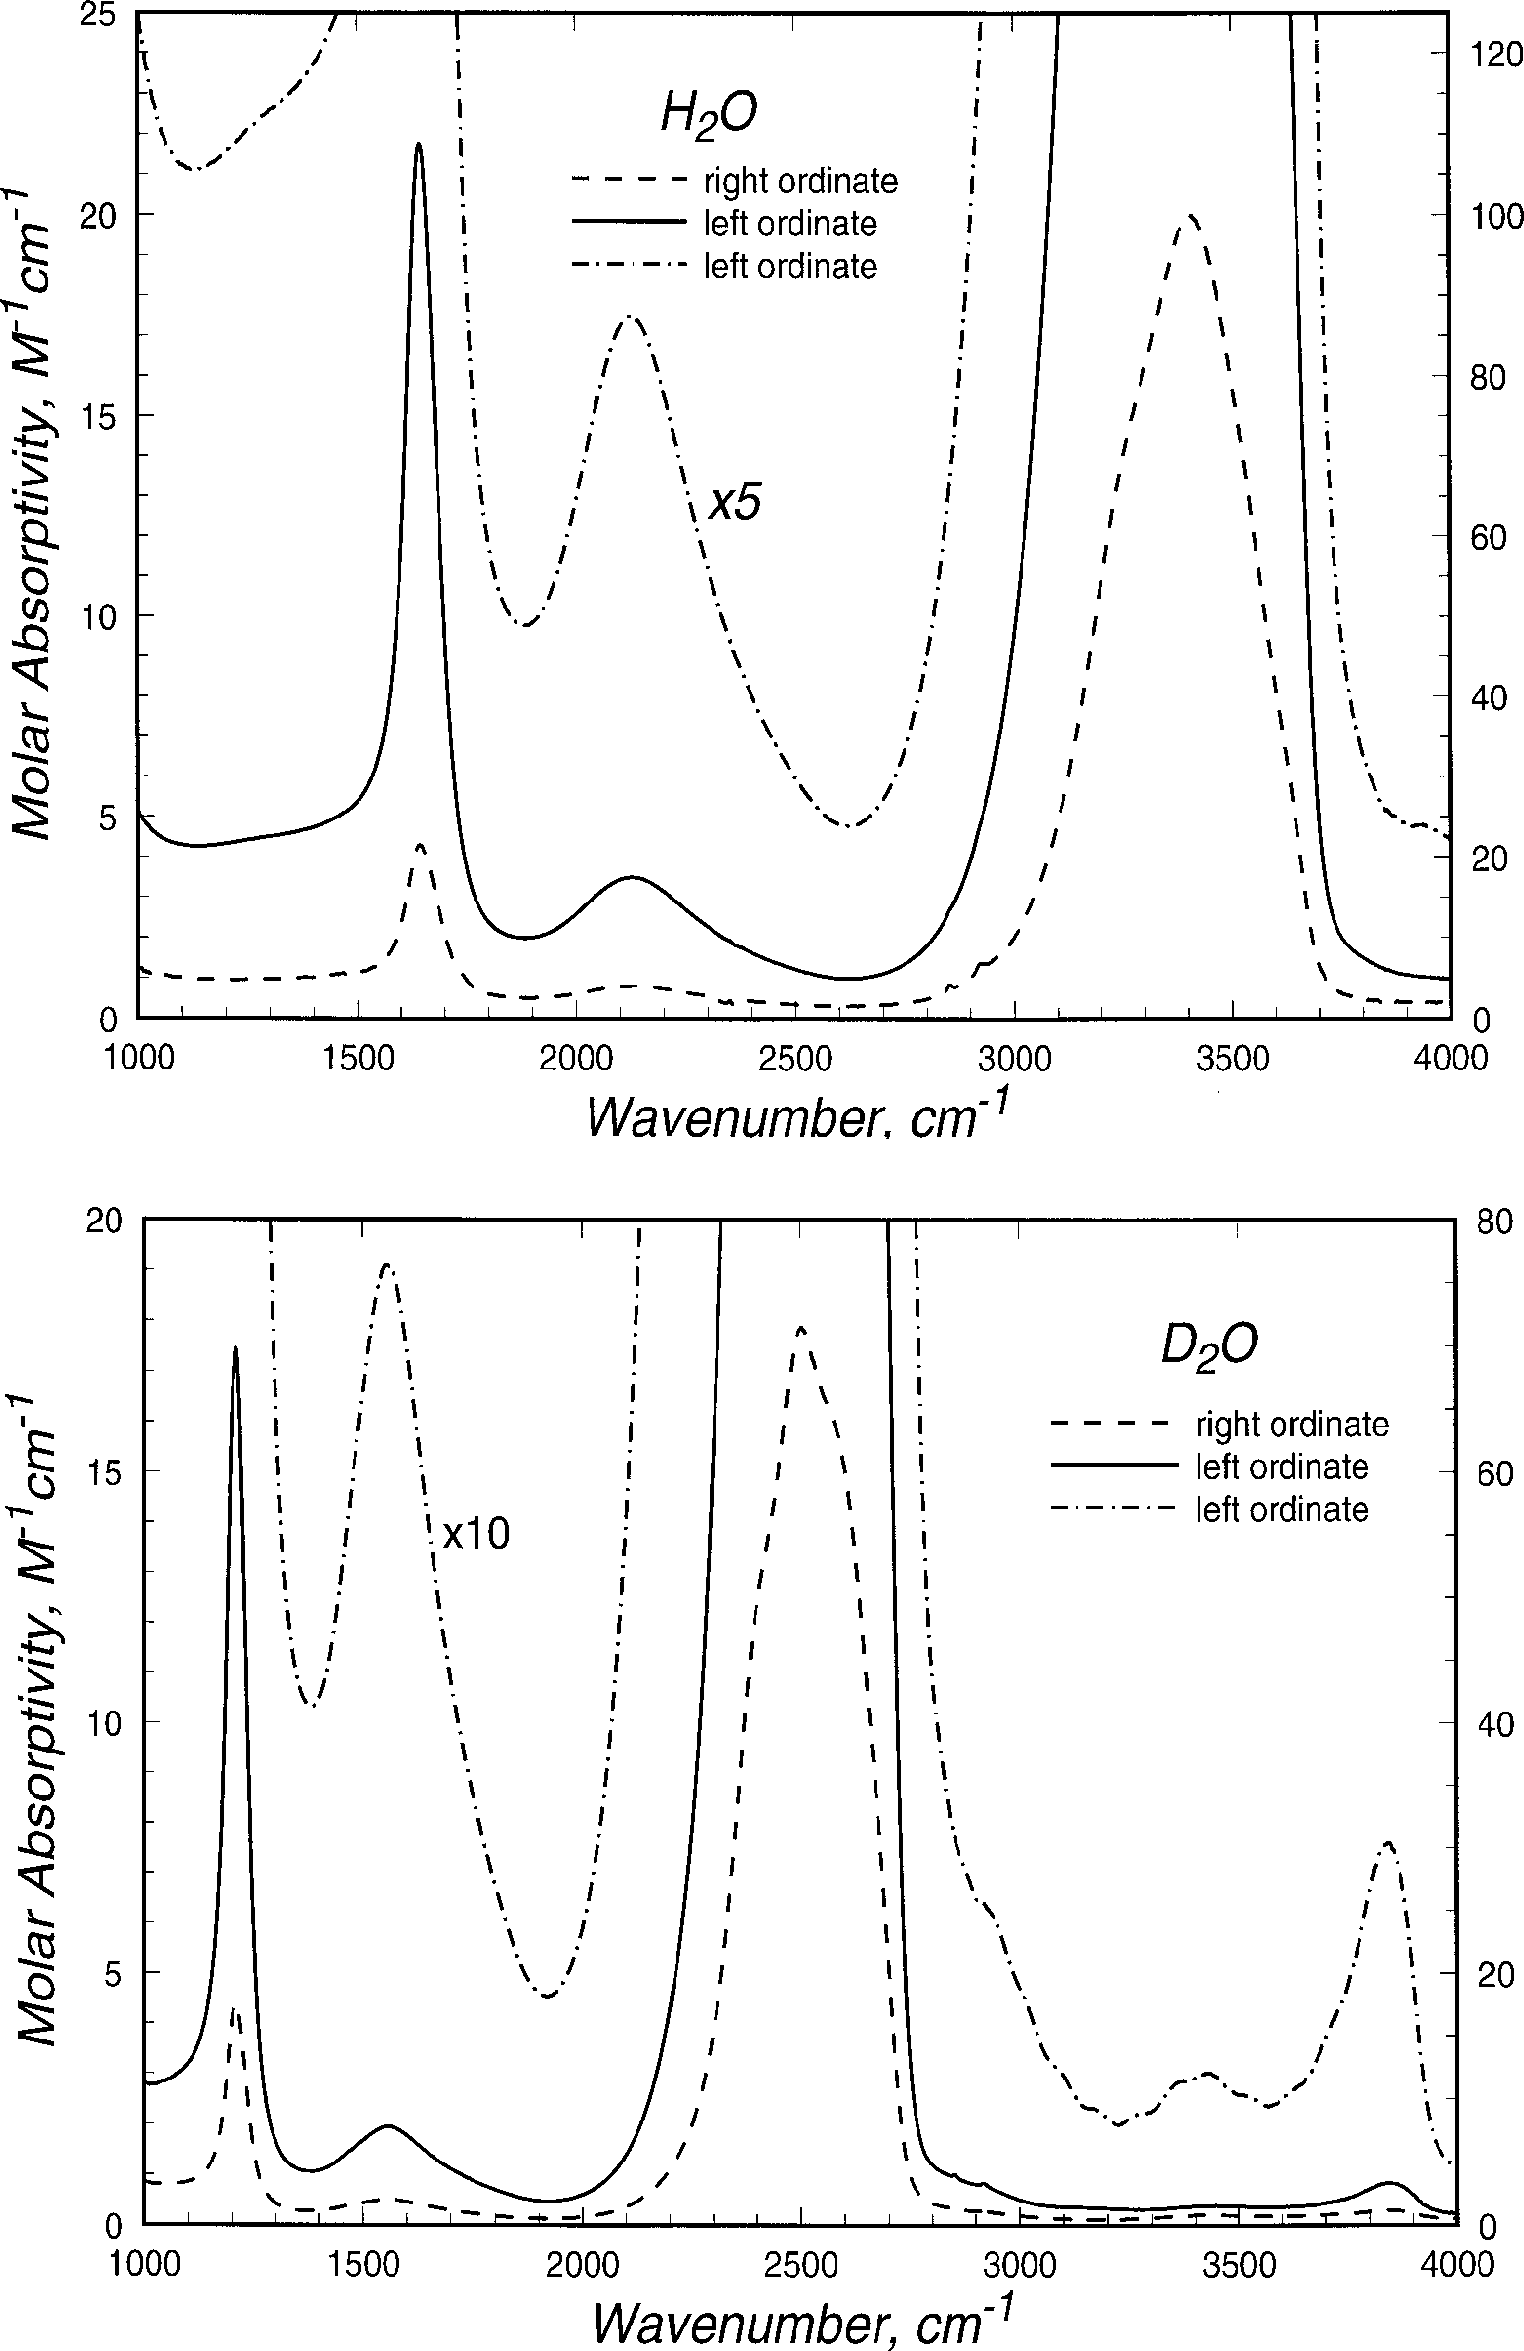
\includegraphics[width=45mm]{img/h2o-d2o.png}
		\end{column}
	\end{columns}
	\footnotetext[1]{\href{https://doi.org/10.1006/abio.1997.2136}{\emph{Anal. Biochem}, \textbf{1997}, \emph{248} (2), 234--245}}
	\vfill
}

\subsection{Halogenované sloučeniny}
\frame{
	\frametitle{}
	\vfill
	\begin{itemize}
		\item Se vzrůstající hmotností halogenu klesá hodnota vlnočtu vazby \ce{C-X}.
		\item 	$\tilde{\nu} = \frac{1}{2\pi c}\sqrt{k\frac{(m_1 + m_2)}{m_1m_2}}$
		\begin{itemize}
			\item k - silová konstanta vazby
			\item $m_1, m_2$ - hmotnosti atomů
		\end{itemize}
		\item V tabulce jsou shrnuty vibrace vazeb \ce{C-X} u alifatických uhlovodíků a vazeb \ce{B-X} v molekulách \ce{MeBX2}.
	\end{itemize}
	\begin{center}
		\begin{tabular}{|l|l||l|l|}
			\hline
			\textbf{Vazba} & \textbf{Vlnočet [cm$^{-1}$]} & \textbf{Vazba} & \textbf{Vlnočet [cm$^{-1}$]}\\\hline
			\ce{C-F} & 1150-1000 & \ce{B-F} & 1365 \\\hline
			\ce{C-Cl} & 800-700 & \ce{B-Cl} & 1018 \\\hline
			\ce{C-Br} & 700-600 & \ce{B-Br} & 965 \\\hline
			\ce{C-I} & 600-500 & & \\\hline
		\end{tabular}
	\end{center}
	\vfill
}

\subsection{NIR}
\frame{
	\frametitle{}
	\vfill
	\begin{itemize}
		\item Oblast 700-2500 nm, tj. 14~000-4~000~cm$^{-1}$.
		\item V této oblasti jsou převážně kombinační vibrace a overtony (vyšší harmonické). Ty poskytují málo intenzivní, široké  pásy, které se často překrývají.
		\item Výhodou je možnost použití běžných optických materiálů (sklo, křemen) a citlivých detektorů.
		\item Voda v této oblasti absorbuje relativně málo, takže ji lze použít jako rozpouštědlo.
		\item Využití v lékařství a zdravotní diagnostice, potravinářském a jiném průmyslu, astronomii, \ldots
		\item Jako měřicí techniky se využívají:
		\begin{itemize}
			\item transmisní technika
			\item difuzně-reflexní technika
			\item transflexe
		\end{itemize}
	\end{itemize}
	\vfill
}

\frame{
	\frametitle{}
	\vfill
	\begin{center}
	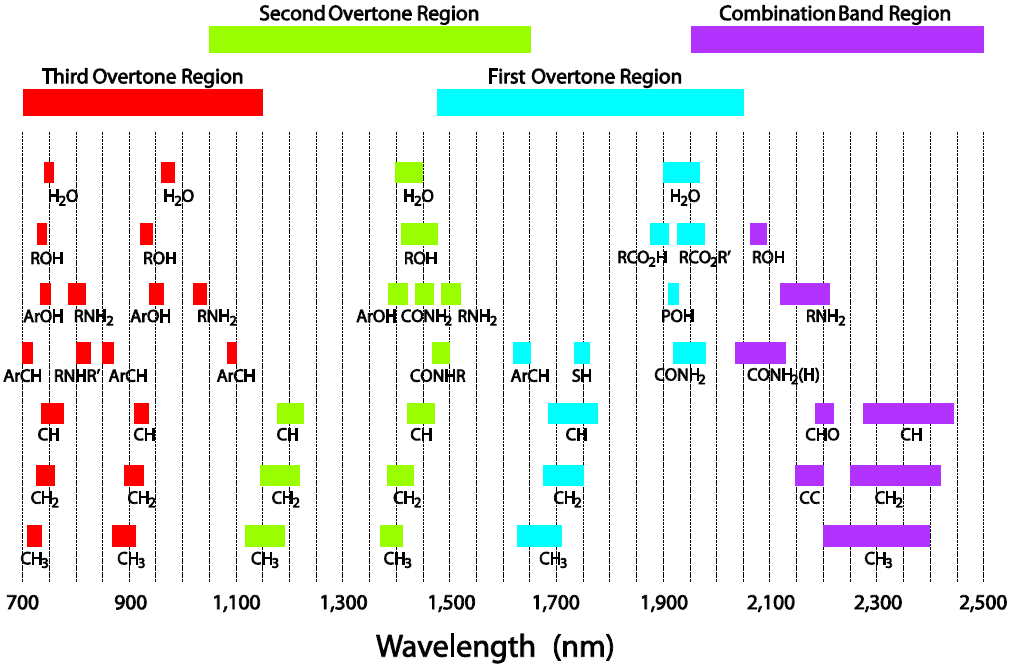
\includegraphics[width=110mm]{img/NIR-bands.png}
	\end{center}
	\vfill
}

\frame{
	\frametitle{}
	\vfill
	\begin{itemize}
	\item NIR spektrum kapalného ethanolu
	\end{itemize}
	\adjincludegraphics[height=.8\textheight]{img/EtOH-NIR.png}
	\vfill
}

\subsection{Ramanova spektroskopie}
\frame{
	\frametitle{}
	\vfill
	\textbf{Ramanova spektroskopie}
	\begin{itemize}
	\item Komplementární metoda k IR spektroskopii
	\item Principem je nepružný rozptyl laserového záření na vzorku
	\item Vhodnější pro nepolární sloučeniny
	\item Lze použít vodu jako rozpouštědlo
	\item Zpravidla užší pásy než v IR spektrech
	\item Jednoduchá příprava vzorku
	\item Měření může komplikovat fluorescence vzorku
	\item Dražší hardware
	\end{itemize}
	\vfill
}

\subsubsection{Studium struktury grafenu}
\frame{
	\frametitle{}
	\vfill
	\begin{columns}
	\begin{column}{0.55\textwidth}
	\begin{itemize}
	\item Pomocí Ramanovy spektroskopie lze studovat kvalitu grafenu a určit počet vrstev vzorku
	\item Pás D (1350~cm$^{-1}$) odpovídá poruchám ve struktuře grafenu.
	\item Pás G (1583~cm$^{-1}$) odpovídá valenčním vibracím vazeb C-C, najdeme ve všech systémech s sp$^2$ uhlíky.
	\item V případě nečistot nebo výskytu náboje na povrchu grafenu, najdeme v blízkosti pásu G i méně intenzivní pás D' (1620~cm$^{-1}$).
	\item 2D pás v oblasti 2500-2800~cm$^{-1}$ (historicky pás G'), nalezneme ho u všech systému s sp$^2$ uhlíky.
	\end{itemize}
	\end{column}
	\begin{column}{0.4\textwidth}
	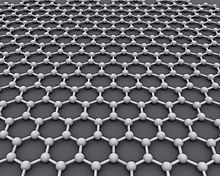
\includegraphics[width=40mm]{img/Graphen.jpg}
	\\
	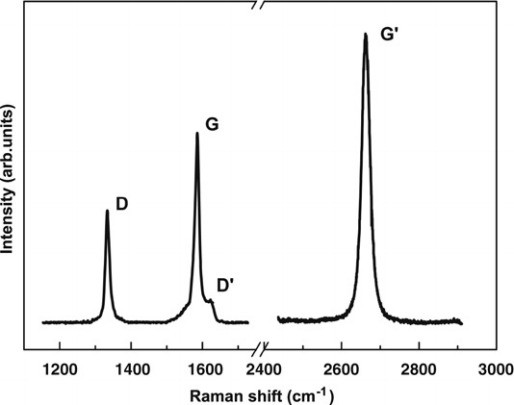
\includegraphics[width=40mm]{img/graphene-Raman.png}
	\end{column}
	\end{columns}
	\vfill
}

\subsection{IR vs Raman}
\frame{
	\frametitle{}
	\vfill
	\textbf{IR vs Raman}
	\begin{columns}[T]
		\column{0.5\textwidth}
		\textbf{Infračervená spektroskopie (IR)}
		\begin{itemize}
			\item Měří absorpci infračerveného záření.
			\item Vibrace musí způsobit změnu dipólového momentu.
			\item Silné pásy:
			\begin{itemize}
				\item O--H
				\item N--H
				\item C=O
			\end{itemize}
			\item Velmi vhodná pro identifikaci polárních funkčních skupin.
			\end{itemize}

			\column{0.5\textwidth}
			\textbf{Ramanova spektroskopie (RA)}
			\begin{itemize}
				\item Měří nepružný rozptyl laserového záření.
				\item Vibrace musí způsobit změnu polarizovatelnosti.
				\item Silné pásy:
				\begin{itemize}
					\item C=C
					\item C$\equiv$C
					\item symetrické vibrace
				\end{itemize}
				\item Velmi vhodná pro málo polární a vysoce symetrická uspořádání.
			\end{itemize}
		\end{columns}
	\vfill
}

\frame{
	\frametitle{}
	\vfill
	\begin{columns}
		\begin{column}{.5\textwidth}
			\begin{alertblock}{IR a Ramanova spektroskopie jsou komplementární metody}
				Vibrace, které jsou v jednom spektru slabé nebo nepozorovatelné, mohou být výrazné ve druhém. Proto se obě metody často používají společně.
			\end{alertblock}
		\end{column}

		\begin{column}{.5\textwidth}
			\begin{figure}
				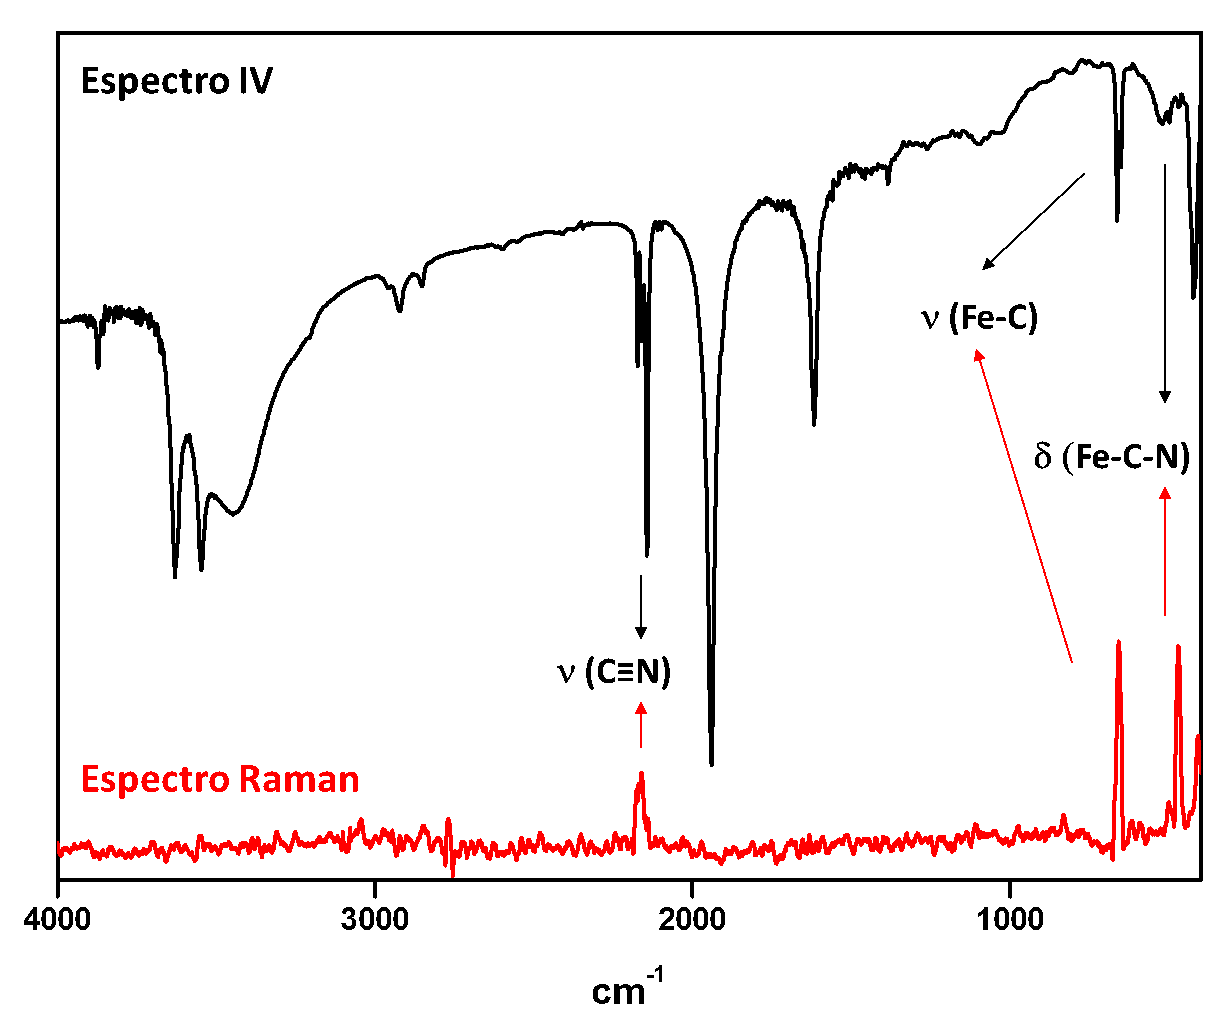
\includegraphics[width=\textwidth]{../img/IR-RA.png}
				\caption*{Infračervené a Ramanovo spektrum kyanidokomplexu železa.\footnote[frame]{\href{https://commons.wikimedia.org/wiki/File:Figura\_3-\_Espectro\_vibracional\_na\_regi\%C3\%A3o\_do\_infravermelho\_e\_espectro\_Raman\_de\_um\_complexo\_pentacianoferrato..png}{Zdroj: Pamyla Santos/Commons}}}
			\end{figure}
		\end{column}
	\end{columns}
	\vfill
}

\section{Interpretace IR spektra za 30 sekund}
\frame{
	\frametitle{}
	\vfill
	\centering
	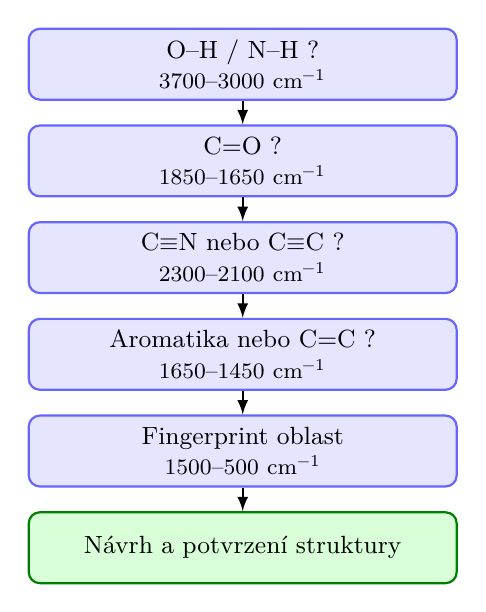
\begin{tikzpicture}[
		node distance=0.3cm, every node/.style={font=\small}, block/.style={ rectangle, rounded corners, draw=blue!60, fill=blue!10, thick, text width=5.2cm, minimum height=0.9cm, align=center }, arrow/.style={ ->, thick, >=latex } ] \node[block] (oh) {O--H / N--H ?\\ \footnotesize 3700--3000 cm$^{-1}$}; \node[block, below=of oh] (co) {C=O ?\\ \footnotesize 1850--1650 cm$^{-1}$}; \node[block, below=of co] (triple) {C$\equiv$N nebo C$\equiv$C ?\\ \footnotesize 2300--2100 cm$^{-1}$}; \node[block, below=of triple] (arom) {Aromatika nebo C=C ?\\ \footnotesize 1650--1450 cm$^{-1}$}; \node[block, below=of arom] (fp) {Fingerprint oblast\\ \footnotesize 1500--500 cm$^{-1}$}; \node[block, below=of fp, fill=green!15, draw=green!50!black] (result) {Návrh a potvrzení struktury}; \draw[arrow] (oh) -- (co); \draw[arrow] (co) -- (triple); \draw[arrow] (triple) -- (arom); \draw[arrow] (arom) -- (fp); \draw[arrow] (fp) -- (result);
	\end{tikzpicture}

	\vspace{0.2cm}
	\textbf{ O--H/N--H $\rightarrow$ C=O $\rightarrow$ C$\equiv$N/C$\equiv$C $\rightarrow$ Aromát/C=C $\rightarrow$ Fingerprint }
	\vfill
}



\section{Kvantitativní analýza}
\frame{
	\frametitle{}
	\vfill
	\begin{itemize}
		\item \emph{Lambert-Beerův zákon} -- $A_\lambda = \epsilon_\lambda l c$
		\begin{itemize}
			\item $A_\lambda$ - absorbance vzorku při vlnové délce $\lambda$
			\item $\epsilon_\lambda$ - absorpční koeficient při vlnové délce $\lambda$. Je charakteristický pro každou sloučeninu.
			\item l - délka kyvety
			\item c - molární koncentrace vzorku
		\end{itemize}
		\item Pro stanovení koncentrace se využívá \emph{kalibrační křivka}.
		\item Pás zvolený pro analýzu musí splňovat několik požadavků:
		\begin{itemize}
			\item Vysoký molární absorpční koeficient
			\item Neměl by se významně překrývat s jinými pásy
			\item Měl by být symetrický
			\item Závislost absorbance na koncentraci by měla být lineární
		\end{itemize}
	\end{itemize}
	\vfill
}

\subsection{Stanovení koncentrace kofeinu v roztoku}
\frame{
	\frametitle{}
	\vfill
	\begin{columns}
		\begin{column}{.8\textwidth}
			\begin{figure}
				\adjincludegraphics[width=\textwidth]{img/caffeine.png}
				\caption*{IR spektrum kofeinu}
			\end{figure}
		\end{column}

		\begin{column}{.2\textwidth}
			\begin{figure}
				\adjincludegraphics[width=\textwidth]{img/caffeine-struct.png}
				\caption*{Struktura kofeinu}
			\end{figure}
		\end{column}
	\end{columns}
	\vfill
}

\frame{
	\frametitle{}
	\vfill
	\begin{columns}
		\begin{column}{.5\textwidth}
			\begin{tabular}{|l|l|}
				\hline
				\textbf{Koncentrace [mg.cm$^{-3}$]} &
				\makecell{\textbf{Absorbance při} \\ \textbf{1656~cm}$^{-1}$} \\\hline
				0 & 0,000 \\\hline
				5 & 0,105 \\\hline
				10 & 0,190 \\\hline
				15 & 0,265 \\\hline
				20 & 0,333 \\\hline
			\end{tabular}
		\end{column}

		\begin{column}{.5\textwidth}
			\begin{figure}
				\adjincludegraphics[width=\textwidth]{img/kalibracni_krivka.png}
			\end{figure}
		\end{column}
	\end{columns}

	\vfill
}

\section{Praktické ukázky}
\frame{
	\frametitle{}
	\vfill
	\adjincludegraphics[height=.85\textheight]{spectra/mocovina-ATR.png}
	\vfill
}

\frame{
	\frametitle{}
	\vfill
	\adjincludegraphics[height=.85\textheight]{spectra/mocovina-SDBS.png}
	\vfill
}

\frame{
	\frametitle{}
	\vfill
	\adjincludegraphics[height=.85\textheight]{spectra/mocovina-nujol-SDBS.png}
	\vfill
}

\frame{
	\frametitle{}
	\vfill
	\adjincludegraphics[height=.85\textheight]{spectra/mocovina-scifinder.png}
	\vfill
}

\frame{
	\frametitle{}
	\vfill
	\adjincludegraphics[height=.85\textheight]{spectra/mocovina-ATR1.png}
	\vfill
}

\frame{
	\frametitle{}
	\vfill
	\adjincludegraphics[height=.85\textheight]{spectra/SO3K-ATR.png}
	\vfill
}


\frame{
	\frametitle{}
	\vfill
	\adjincludegraphics[height=.85\textheight]{spectra/SO3K-ATR1.png}
	\vfill
}

\frame{
	\frametitle{}
	\vfill
	\adjincludegraphics[height=.85\textheight]{img/Ph3SiOH-struct.png}
	\vfill
}

\frame{
	\frametitle{}
	\vfill
	\adjincludegraphics[height=.85\textheight]{img/Ph3SiOH-struct2.png}
	\vfill
}

\section{Literatura a odkazy}
\frame{
	\frametitle{}
	\vfill
	\begin{enumerate}
	\item STUART, Barbara. \emph{Infrared spectroscopy: fundamentals and applications.} Hoboken, NJ: J. Wiley, 2004. ISBN 9780470854280.
	\item COATES, John. Interpretation of Infrared Spectra, A Practical Approach.\emph{ Encyclopedia of Analytical Chemistry} [online]. Chichester, UK: John Wiley \& Sons, 2006 [cit. 2017-05-18]. DOI: 10.1002/9780470027318.a5606. ISBN 0470027312. Dostupné z: http://doi.wiley.com/10.1002/9780470027318.a5606
	\item \href{http://sdbs.riodb.aist.go.jp/sdbs/cgi-bin/cre\_index.cgi}{Spectral Database for Organic Compounds} -- http://sdbs.riodb.aist.go.jp/sdbs/cgi-bin/cre\_index.cgi
	\item  \href{http://webbook.nist.gov/chemistry/}{NIST Webbook Chemistry} -- http://webbook.nist.gov/chemistry/
	\end{enumerate}
	\vfill
}

\frame{
	\vfill
	\centering \Huge
	\textbf{Děkuji za pozornost} \\[2ex]

	\large
	Zdeněk Moravec\\
	hugo@chemi.muni.cz \\
	\vfill
}

\end{document}